\chapter{Preliminaries}
\label{ch:preliminaries}
\newpage

\section{RDF Model}
The "Semantic Web" \cite{W3C:SemanticWebTerm:Online} term  has appeared during the transformation process of Web Development from "Web of documents" to "Web of data", similar to those data are found in databases. W3C defines it as "the Web of linked data" . {\it Figure \ref{Fig:semanticWebStack} describes the Semantic Web Stack, proposed by W3C. It can be seen, that it contains several technologies to enable users of creating their own data stores on web, building vocabularies, and enforcing processing rules on such data.   
\vspace{5mm} %5mm vertical space
\par
In order to make data more and machine-readable, RDF Model has been proposed. RDF Model is considered as a model for data interchange in the new generation of web stack (called Semantic Web).   
	\begin{figure}[ht]
	\begin{center}
		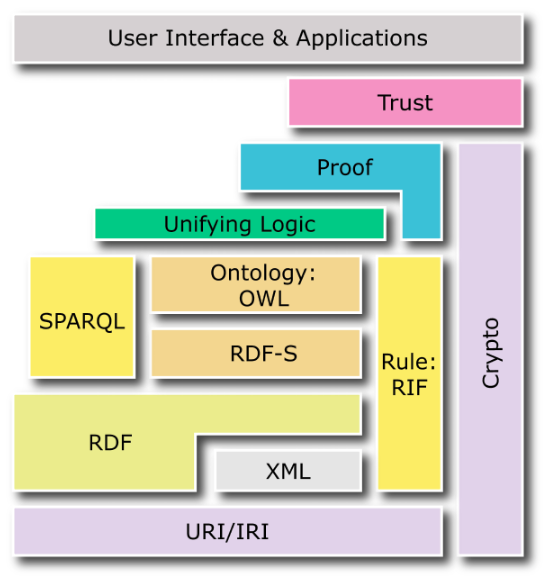
\includegraphics[scale=0.5,angle=0]{images/semanticWebStack}
		\caption{The Semantic Web Stack \cite{Bratt2007}}
		\label{Fig:semanticWebStack}
	\end{center}
\end{figure}

\section{Parsing Methodologies}
If you have a chance to look to the red book of the compiler, then you absolutely know that there are several methods for building parsers.    
\section{ANTLR Parser Generator }
ANTLR is an handy tool and easy way to have a parser. It is an parser generator where an normal user can build his own language's parser without much works. The basic principle used by ANTLR is define language's rules which draws the syntax and the semantic of the language the parser build for. 

\vspace{5mm} %5mm vertical space
\par
 As has been previously discussed, the compiler has two main subsystems: lexer and parser. Both lexer and parser are needed to have their rules defined in ANTLR grammar file.  


















